\subsection{Teleconnections}
\label{sub:tele}
It has long been recognised that global atmospheric weather systems are linked on intraannual and longer timescales, which was first noted and recorded in David Crantz’s
\textit{The History of Greenland(1767):\\
“It has been many times remarked, that the weather in Greenland is just the reverse to that in Europe; so that when the temperate climates are incommoded with a very hard winter, it is here uncommonly mild, and vice versa”.}\cite{Kidston2009}\\

In the 1920s, more extensive studies on atmospheric linkages and oscillations were carried out by Sir Gilbert Walker. Three patterns of pressure anomalies were noted and named the \textit{North Atlantic Oscillation} (NAO), \textit{North Pacific Oscillation} (NPO) and \textit{Southern Oscillation}. The latter SO relates to a see-saw like oscillation of sea level pressure in different sectors of the Pacific Ocean named the Walker circulation in his honour many years later, which is closely related to the well known El Nino Southern Oscillation (ENSO) \cite{Gong1999} \cite{WALKER1923}. \\

In this connection, the term teleconnection in atmospheric science is commonly used to describe climatic linkages, either directly or indirectly, between geographically separated regions, which might be thousands of kilometres apart from each other. The word teleconnection was first used in the mid 1930s \cite{Angstrom1935} and has not established itself in climatic literature  until the 1980s. Generally, these linkages can proceed on interannual?? as well as on decadal time scales and are mostly associated with oscillations. Any phenomena that shows fluctuations around a mean value in some kind of periodic way is named an oscillation. 
 In atmospheric science, these anomalies  could principally emerge in all possible kinds of climatic variables, such as sea surface temperatures, zonal winds,  pressure fields etcetera(etc.). The terms anomaly and fluctuation are thereby associated with the deviation of the climatic field from its respective mean annual cycle.
 
  Thus, teleconnections are commonly characterised by simultaneous fluctuations of a climatic field of opposite or even the same sign within separated areas. The name basically refers to the fact that these either positive or negative correlations suggest, that some kind of information is transported between the distant regions throughout the atmosphere. By employing statistical analysis techniques, such as correlation and regression maps or empirical orthogonal function analysis, on  observed interannual??? and decadal?? variability of sea level pressure, zonal wind or geopotential height fields, these teleconnection patterns can be identified[????].\\
It shows up, that these patterns occur around the globe, as well on the northern hemisphere as well as on the southern hemisphere....\\\\


 






	\subsection{AO}


	\subsubsection{Southern Annular Mode (SAM)}
	The question is, whether there are other oscillations like SO,NAO,NPO????
	In 1928, Sir Gilbert Walker stated: \textit{Just as in the North Atlantic there is a pressure opposition between the Azores and Iceland,... ,there is an opposition between the high pressure belt across Chile and the Argentine on the one hand, and the low pressure area of Weddell Sea and the Bellingshausen Sea on the other} \cite{Gong1999}
	However, the scarcity of observational data about this region did not allow for more profound research on this supposed oscillation. \\
	In the 1980s, when more data about the Southern Hemisphere became available and more analyses were carried out, the existence of such an oscillation in the mid and high southern latitudes was confirmed and named the \textit{Antarctic Oscillation} (AO) [??].
	The Antarctic Oscillation, also known as the Southern Annular Mode (SAM), describes the most dominant mode of extratropical climate variability on timescales ranging from interannual to intraseasonal timescales over the Southern Hemisphere \cite{Thompson2000}. By convention, it is associated with an alternation of masses between the mid and the high latitudes resulting in higher pressure anomalies over the mid-latitudes and lower pressure anomalies over Antarctica in its positive phase and vice versa in its negative phase. For illustration, figure \ref{fig:SAM_low_high} shows polarstereographic plots of the ERA-Interim monthly geopotential height anomalies for a  negative phase (February 2002) and a positive phase (May 1989). 

\begin{figure}
		\centering
		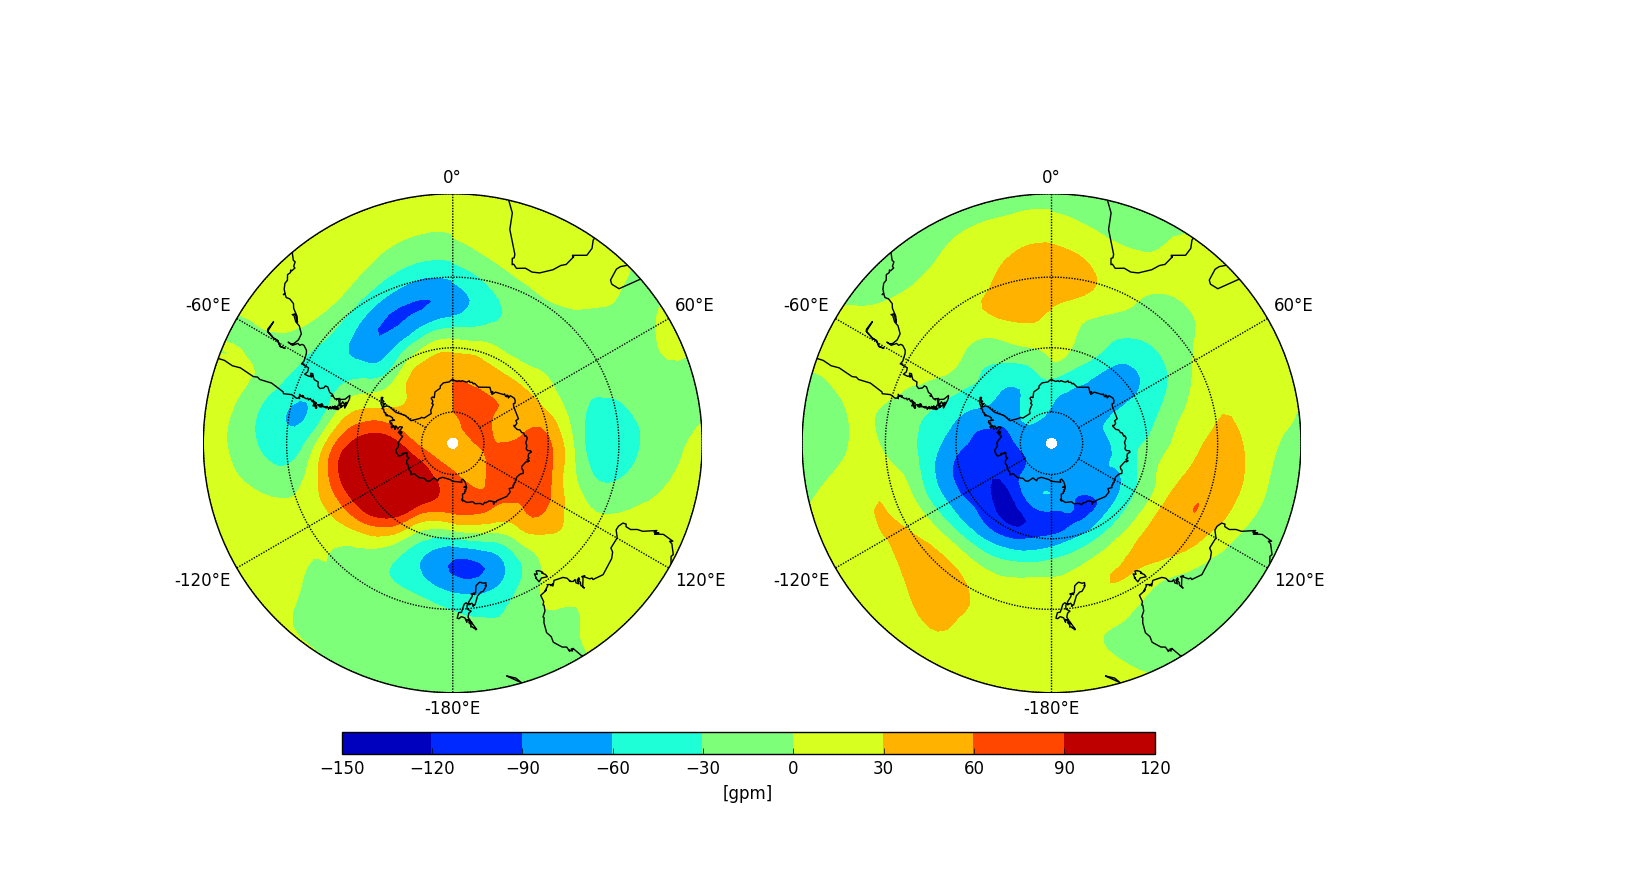
\includegraphics[scale=0.4]{pictures/SAM_low_high.png}
		\caption{left February 2002 right May1989}\label{fig:SAM_low_high}
		
\end{figure}	
	
	
	
	Furthermore,figure \ref{fig:correlation_sam} depicts the crosscorrelation coefficients of monthly zonally averaged geopotential height anomalies of the 700\,hPa pressure level in the Southern Hemisphere using ERA-Interim reanalysis data. The SAM manifests itself in the strong and significant negative correlation down to -0.76 between the midlatitudes (40$^\circ$S) and the high-latitudes(60-70$^\circ$S) \cite{Gong1999}, which implies that increasing pressures above the mid-latitudes are typically accompanied by decreasing pressures above the high latitudes and vice versa.\\
	For characterising the current state of the SAM in a respective month several SAM-indices have been defined over time. The first and maybe most simplest definition of a SAM index (SAMI) using reanalysis data was given by Gong and Wang (1999) \cite{Gong1999}:
	\begin{align}\label{eq:Gong}
		\text{SAMI}=P^{*}_{40^\circ S}-P^{*}_{65^\circ S},
	\end{align}
where $P^{*}_{40^\circ S}$ and $P^{*}_{65^\circ S}$ stands for the normalised zonal mean SLP of 40$^\circ$S and 65$^\circ$S for every month respectively. A slightly different definition is given by Nan and Li (2003) \cite{Nan2003}, who used 70$^\circ$S zonal mean SLP  $P^{*}_{70^\circ S}$ instead of  $P^{*}_{65^\circ S}$ by reason of supposedly stronger negative correlations in the zonally-mean? SLP between 40$^\circ$S and 70$^\circ$S compared to 40$^\circ$S and 65$^\circ$S. In order to examine the reliability of such reanalysis-based SAMI before the satellite era, station based indices have been introduced, for instance by  Marshall \cite{Marshall2003}, who uses mean SLP observations from six stations located at 40$^\circ$S and 65$^\circ$S respectively to provide a proxy zonal mean.\\
A more sophisticated and commonly used definition of the SAMI is given by the first principal component of the Leading Empirical Orthogonal Function as described in chapter \ref{subsec:EOF}. Many more indices with their individual strengths and weaknesses have been defined over the last years and it also points out that time series of differently defined SAMI are strongly and significantly correlated with each other.\cite{Ho2012a}\\

To get a notion of the coarse shape of the SAM, Figure \ref{fig:ind_mslp_regress} illustrates a linear regression of the time series of monthly zonal mean ERA-Interim geopotential height anomaly fields onto the standardized  time  series of monthly SAMI calculated according to equation \ref{eq:Gong} for the NOAA 20th-Century Reanalysis data [taken fromwebsite, oder lieber IERA ???]. Apparently, an increase of the SAMI by its standard deviation is typically accompanied by a decrease of the 700\,hPa height level of more than 20\,gpm over the entire Antarctic continent down to 50\,gpm over the Amundsen sea in western Antarctica, whereas over the mid-latitudes an overall increase with maxima up to 30\,gpm over the three oceans can be observed. Thus, despite the fact that the term "annular"  suggests that the SAM occurs in a zonally? symmetric and ring-shaped pattern, a strong nonsymmetric wave-3-pattern over the mid-latitudes is detectable, which is presumably closely connected to planetary Rossby-waves.  Fogt ....
As model studies suggested the SAM owes its existence to internal atmospheric dynamics



	
\subsubsection{Impacts on Southern Hemisphere('s) Climate}
Several studies have demonstrated that the SAM has an important and significant influence on the climate system over the entire southern hemisphere[???].\\
 Due to an increase of the meridional pressure gradient  $\frac{\partial p}{\partial y}$ between the mid and the high-latitudes, a positive SAM phase is associated with a strengthening of the westerly wind belt. This fact can be explained by considering the geostrophic equation
\begin{align*}
	fu=\frac{1}{\rho}\frac{\partial p}{\partial y},
\end{align*}
which describes the proportional relationship between the zonal wind speed $u$ and the meridional pressure gradient $\frac{\partial p}{\partial y}$ for a frictionless fluid on a rotating sphere with the hydrostatic and steady state approximation being made. The parameter $f$ describes the coriolis parameter and $\rho$  the air density.\\
 A regressions  between the SAM index and wind speed wind direction \cite{Lovenduski2005}, as done in figure \ref{dd}, indicates that the anomalously strong pressure gradient during  a positive SAMI acts to significantly strengthen the westerly winds at around 55$^\circ$S, and to weaken the westerlies at around 35$^\circ$S (easterly anomaly), by \SI{0.9}{\metre\per\second} in certain regions, resulting in a shift of the westerly wind belt towards Antarctica. In this connection, a southward shift of the Antarctic circumpolar stormtrack has been recognised \cite{Thompson2000},\cite{Gillett2006}, which acts as a relatively narrow zone, in which extratropical cyclonic storms travel driven by the prevailing winds. It has been shown that these  changes in atmospheric circulation impact other components of the climate system in the Southern Hemisphere as well\cite{Hall2002}.\\
 
It has been shown, that the frictional transfer of momentum at the air–sea interface has affects ocean circulation in the southern hemisphere. Westerly wind anomalies in the positive SAM phase increase northward Eckman transport of surface water between 45$^\circ$S and 65$^\circ$S and easterly wind anomalies induce stronger southward Eckman transport between 30$^\circ$S and 45$^\circ$S. Mass conservation induces that the divergence around the Antarctic coast implies stronger warm and nutrient-rich deep water upwelling, which favours biological productivity, whereas the convergence around 45$^\circ$S causes  stronger surface water downwelling \cite{Lovenduski2005}. Figure \ref{qq} depicts the regression between the SAMI and chlorophyll concentration and indicates a strengthening around the Antarctic coast of production as a response to increasing SAMI and( a weakening around 45$^\circ$S).  Additionally, a more intense circumpolar current may be associated with an increasing SAMI \cite{Hall2002}\\

Analyses about the effect of an increasing SAMI on the sea-ice extend in the Southern ocean suggest that the main response results in a decrease of ice in the Weddell Sea, and an increase in the Ross Sea, Amundsen Sea and parts of the Pacific sector \cite{Lefebvre2004}.\\

The previously described upwelling effect of  warm deep water around the Antarctic coast has shown to be connected to stronger ice shelf basin melt, which possibly acts as a driver for the destabilisation of the Antarctic Ice Shelf \cite{Greene2017}.
Other studies demonstrated that a positive SAM phase is associated with anomalously cold surface temperatures over most of Antarctica and warming over the Antarctic Peninsula. Furthermore, decrease in zonal SST in the circumpolar region, increases in the subtropics  \cite{Hall2002} and significant regional warmings over southern Chile and Argentina, over Tasmania and south- eastern Australia over the South Island of New Zealand have been observed in connection with a increasing SAMI \cite{Gillett2006}.\\

Additionally to the previous aspects, several other studies have been published about the SAM's influence on other earth system components, such as carbon cycle \cite{Butler2007} and precipitation over the Southern Hemisphere \cite{Silvestri2003}.





 
	
	
	\begin{figure}
		\centering
		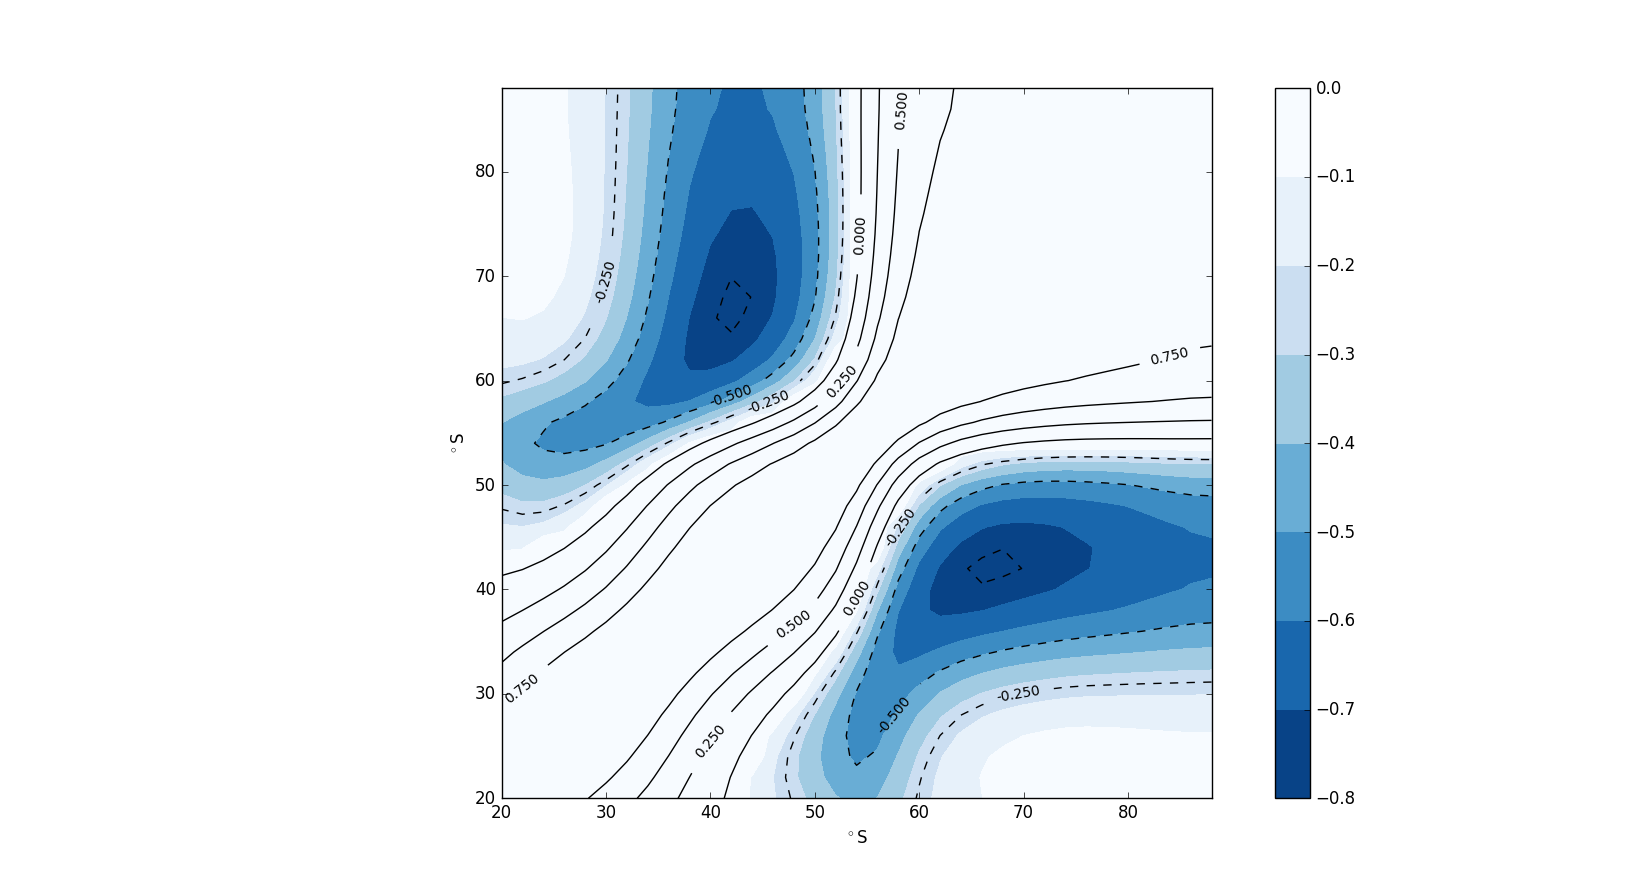
\includegraphics[scale=0.4]{pictures/correlation_IERA.png}
		\caption{Crosscorrelation coefficients of zonal-averaged Sea Level Pressure (SLP) anomalies in the SH using} \label{fig:correlation_sam}
	\end{figure}
	
	\begin{figure}
		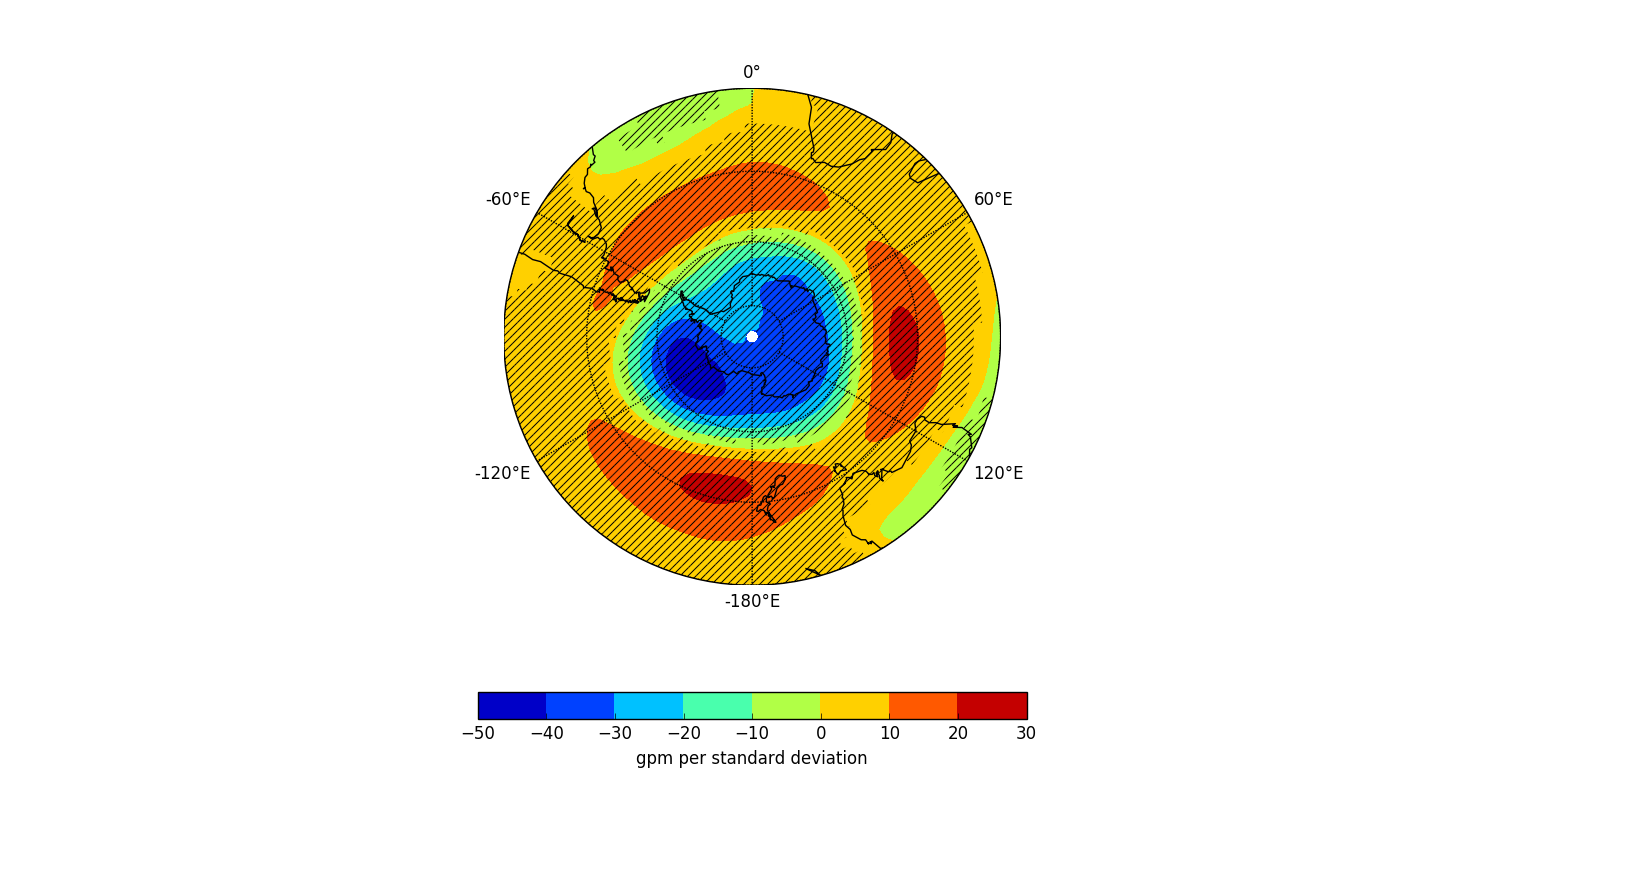
\includegraphics[scale=0.5]{pictures/regression_all.png}
		\caption{jj} 
	\end{figure}
	
%	\begin{figure}
%		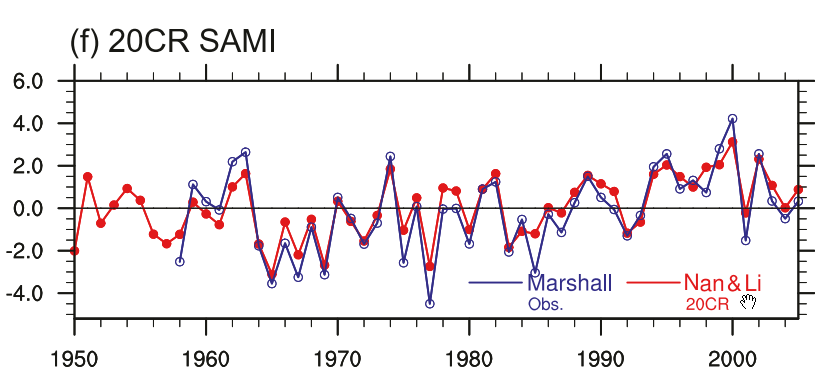
\includegraphics[scale=0.5]{pictures/SAM_index_20CR.png}
%		\caption{(20 CR taken from \cite{Zheng2013a}} 
%	\end{figure}
%	
%	\begin{figure}
%		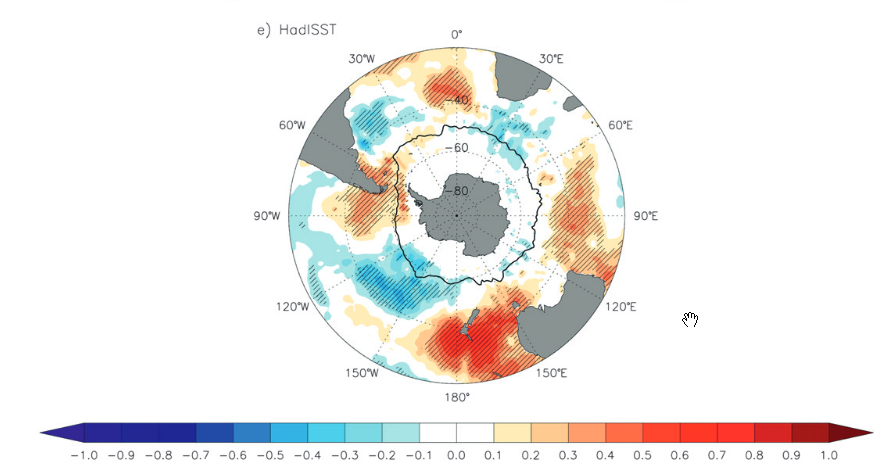
\includegraphics[scale=0.5]{pictures/SST_corr_SAMindex.png}
%		\caption{taken from \cite{Screen2009}}
%	\end{figure}
%	
%	\begin{figure}
%		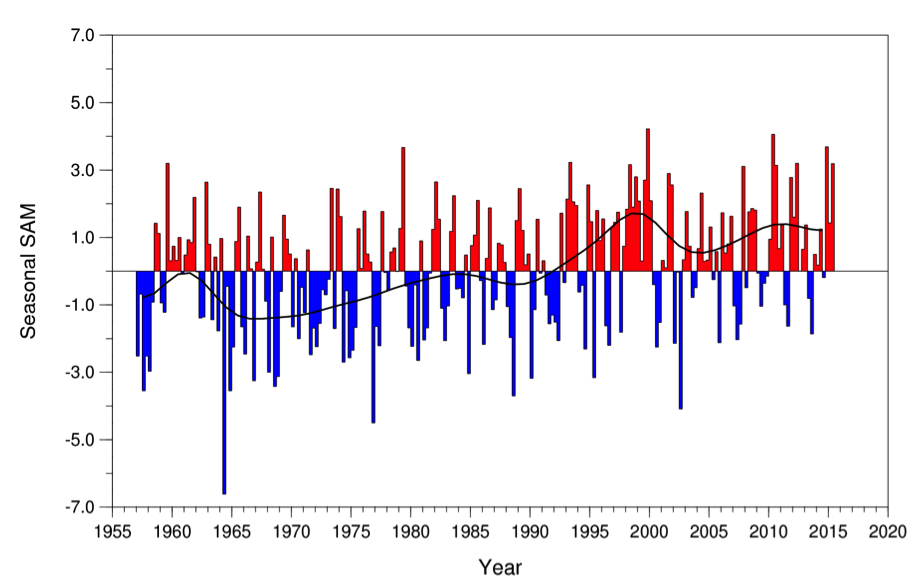
\includegraphics[scale=0.5]{pictures/station_based_SAM}
%		\caption{taken from \cite{station_based_SAM}}
%	\end{figure}
	
	\begin{figure}
		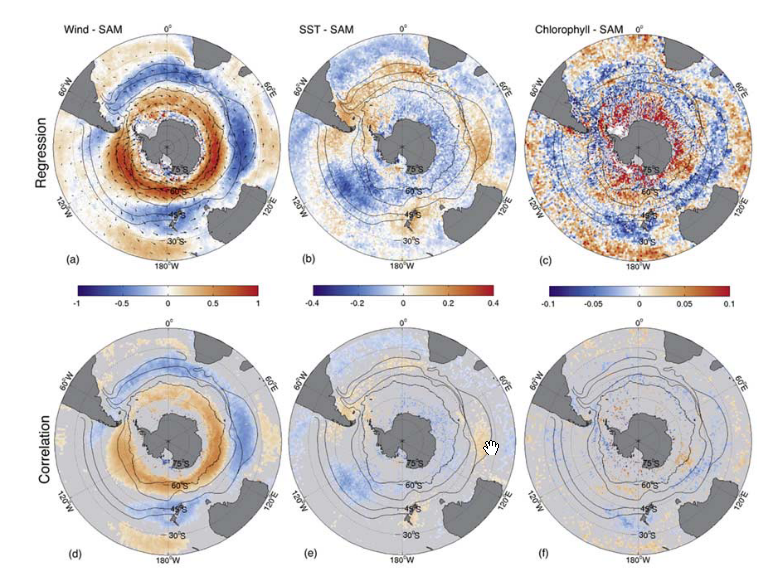
\includegraphics[scale=0.75]{pictures/SAM_regression_SST_wind.png}
		\caption{taken from \cite{Lovenduski2005}}
	\end{figure}
	
	
	\subsection*{mechanism}
	\subsection{drivers of the sam}
	external forcings ozone greenhouse gas recovery
	evolution over millenia